%https://www.overleaf.com/learn/latex/Creating_a_document_in_LaTeX
%https://oeis.org/wiki/List_of_LaTeX_mathematical_symbols
\documentclass[12pt]{report}
\usepackage{graphicx}
\graphicspath{ {./../Output/} {./../} }

\title{CS 440: Probabilistic Search}
\author{Steven Nguyen \& Kyra Kennedy}
\date{10 April 2021}

\begin{document}

\begin{titlepage}
\maketitle
\end{titlepage}

\section*{Abstract}
In this project, we demonstrated basic techniques of supervised learning and computer vision in Python.

\section*{Academic Integrity}
-

\section*{The Basic Coloring Agent}
\begin{figure}
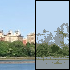
\includegraphics[width=.5\textwidth]{Basic Agent Prediction}
\caption{In the above picture, the left is the training data and the right is the prediction}
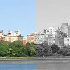
\includegraphics[width=.5\textwidth]{Test Image}
\caption{In the above picture, the left is the training data and the right is the test data}
\end{figure}
The final result isn't great. Though it has the water, sky, and tree colors correctly placed, there many problems. The main problems were that we used 5 k-means, so we can only have 5 of the many colors; because we used patches of 3x3, we can't color the edge of the image; and because we only used 3x3 patches, each test pixel does not have that much information to work off of.\\
We could measure the quality of the final result using P-Norms between the actual image and the prediction. We implemented checking the L2 Norm in Agent.check\_prediction(). This prediction is somewhat numerically satisfying, but still, not great.

\end{document}